\documentclass[12pt]{spieman}  % 12pt font required by SPIE;
%\documentclass[a4paper,12pt]{spieman}  % use this instead for A4 paper
\usepackage{amsmath,amsfonts,amssymb}
\usepackage{graphicx}
\usepackage{setspace}
\usepackage{tocloft}
\usepackage{hyperref}
\usepackage{graphicx}
\usepackage{float}
\usepackage{wrapfig}
\title{Information Retrieval - Submission Report \\Project N.14: Art For Sale}

\author{Jeferson Morales Mariciano}
\author{Filippo Piloni}
\affil{Università della Svizzera italiana, Faculty of Informatics, Lugano, Switzerland}

\renewcommand{\cftdotsep}{\cftnodots}
\cftpagenumbersoff{figure}
\cftpagenumbersoff{table} 
\begin{document}

\begin{wrapfigure}{l}{0.25\textwidth}
    
\includegraphics[width=0.25\textwidth, trim={0cm 0cm 0cm 7cm}]{USI_logo.png}
\end{wrapfigure}

\maketitle
\tableofcontents
\newpage

\begin{spacing}{1}   % use double spacing for rest of manuscript

    \section{Introduction}
    The Information Retrieval course project \textit{"ArtForSale"} aims to be a working prototype of an
    information retrieval system for a specific task: to display for-sale artworks from art selling related
    websites listed in Section \ref{sec:websites}.
    The system has around $\approx 8,500$ indexed documents for searching, browsing and presented through a
    user-friendly and intuitive interface, further details in UI/UX Section \ref{sec:ui}.
    The source code repository of the project is linked in Section \ref{sec:references}.
    
    \subsection{Dowload}
    The complete code exceeded the size allowed by iCorsi. For this reason, the repository can be found at \url{https://github.com/JekxDevil/IR-ArtForSale}

    \subsection{Websites}\label{sec:websites}
    The following websites were chosen for the project based on availability of data, ease of scraping and
    low restrictions regarding policies and terms of use to scrape documents i.e. \textit{robots.txt} rules:

    \begin{itemize}
        \item \url{www.artsy.net}
        \item \url{www.artfinder.com}
        \item \url{www.saatchiart.com}
    \end{itemize}

    The cumulative number of documents gathered from the above websites is around $\approx 8,500$ stored in
    \textit{results.json} file containing the list of samples in JSON format.
    Further information concerning the scraping process and implementation is discussed
    in Crawler Section \ref{sec:crawling}.

    \subsection{Features}
    The course project requires 2 additional categorized features to be implemented besides
    the retrieval system:
    1 each from simple and complex group features.\\
    The \textit{Art For Sale} project implements 2 + 1 bonus additional simple features:

    \begin{itemize}
        \item Simple
              \begin{itemize}
                  \item \textbf{Result presentation}:
                        results should be presented in a tabular format so that many results could be
                        seen at the same time.
                        Each table cell should contain appropriate information for your project.
                  \item \textbf{Filtering}:
                        in addition to being able to search by title, an user should be able to filter the
                        results based on at least 3 relevant attributes for your project.
              \end{itemize}
        \item Complex
              \begin{itemize}
                  \item \textbf{Automatic recommendation}:
                        In addition to the relevant search results pertaining to the user query,
                        the user should also be suggested "similar" products based on, say,
                        category, description, price etc.
                        The ordering among the recommended items is not important.
                        However, you should mention how did you arrive at the recommendations.
                        For this purpose, you can use any open-source recommenders available.
              \end{itemize}
    \end{itemize}

    Shown results are sorted in descending order of relevance from left to right in the tabular view.\\
    Implementation details are on Architecture, Recommender and Filtering Sections
    \ref{sec:architecture}, \ref{sec:recommender}, \ref{sec:filtering}.\\
    Moreover, by exploiting the automatic recommandation feature implemented using category tags
    and the filtering feature to filter them,
    the \textbf{Results clustering} complex feature was tackled by allowing to group the results
    into topics based on category tags.
    Though, a negative filter to exclude documents based on categories was not added,
    thus partially implementing another extra feature.\\

    %%%%%%%%%%%%%%%%%%%%%%%%%%%%%%%%%%%%%%%%%%%%%%%%%%%%%%%%%%%%%%%%%
    \section{Architecture}\label{sec:architecture}

    The \textbf{Information Retrieval System} has capabilities limited to a
    \textbf{TIS}\footnote{Text Information System}
    with \textbf{Text retrieval}.\\
    The \textbf{Text Access} part helping users to retrieve the right information at the right time,
    is structured by connecting the system with users in both modes:
    \begin{itemize}
        \item \textbf{Pull}: user takes initiative to fetch ad-hoc relevant information from the system,
              which offers \textbf{querying} and \textbf{browsing} capabilities.
              It satisfies \textbf{short-term needs}.
        \item \textbf{Push}: system takes initiative and has good knowledge of what are the user's
              \textbf{long-term needs} of information throughout the filtering and recommendation system
              using \textbf{browsing traces} to model the behavior of the user.
    \end{itemize}

    \begin{figure}[H]
        \centering
        \caption{Search Engine Architecture of \textit{ArtForSale} project}
        \label{fig:architecture}
        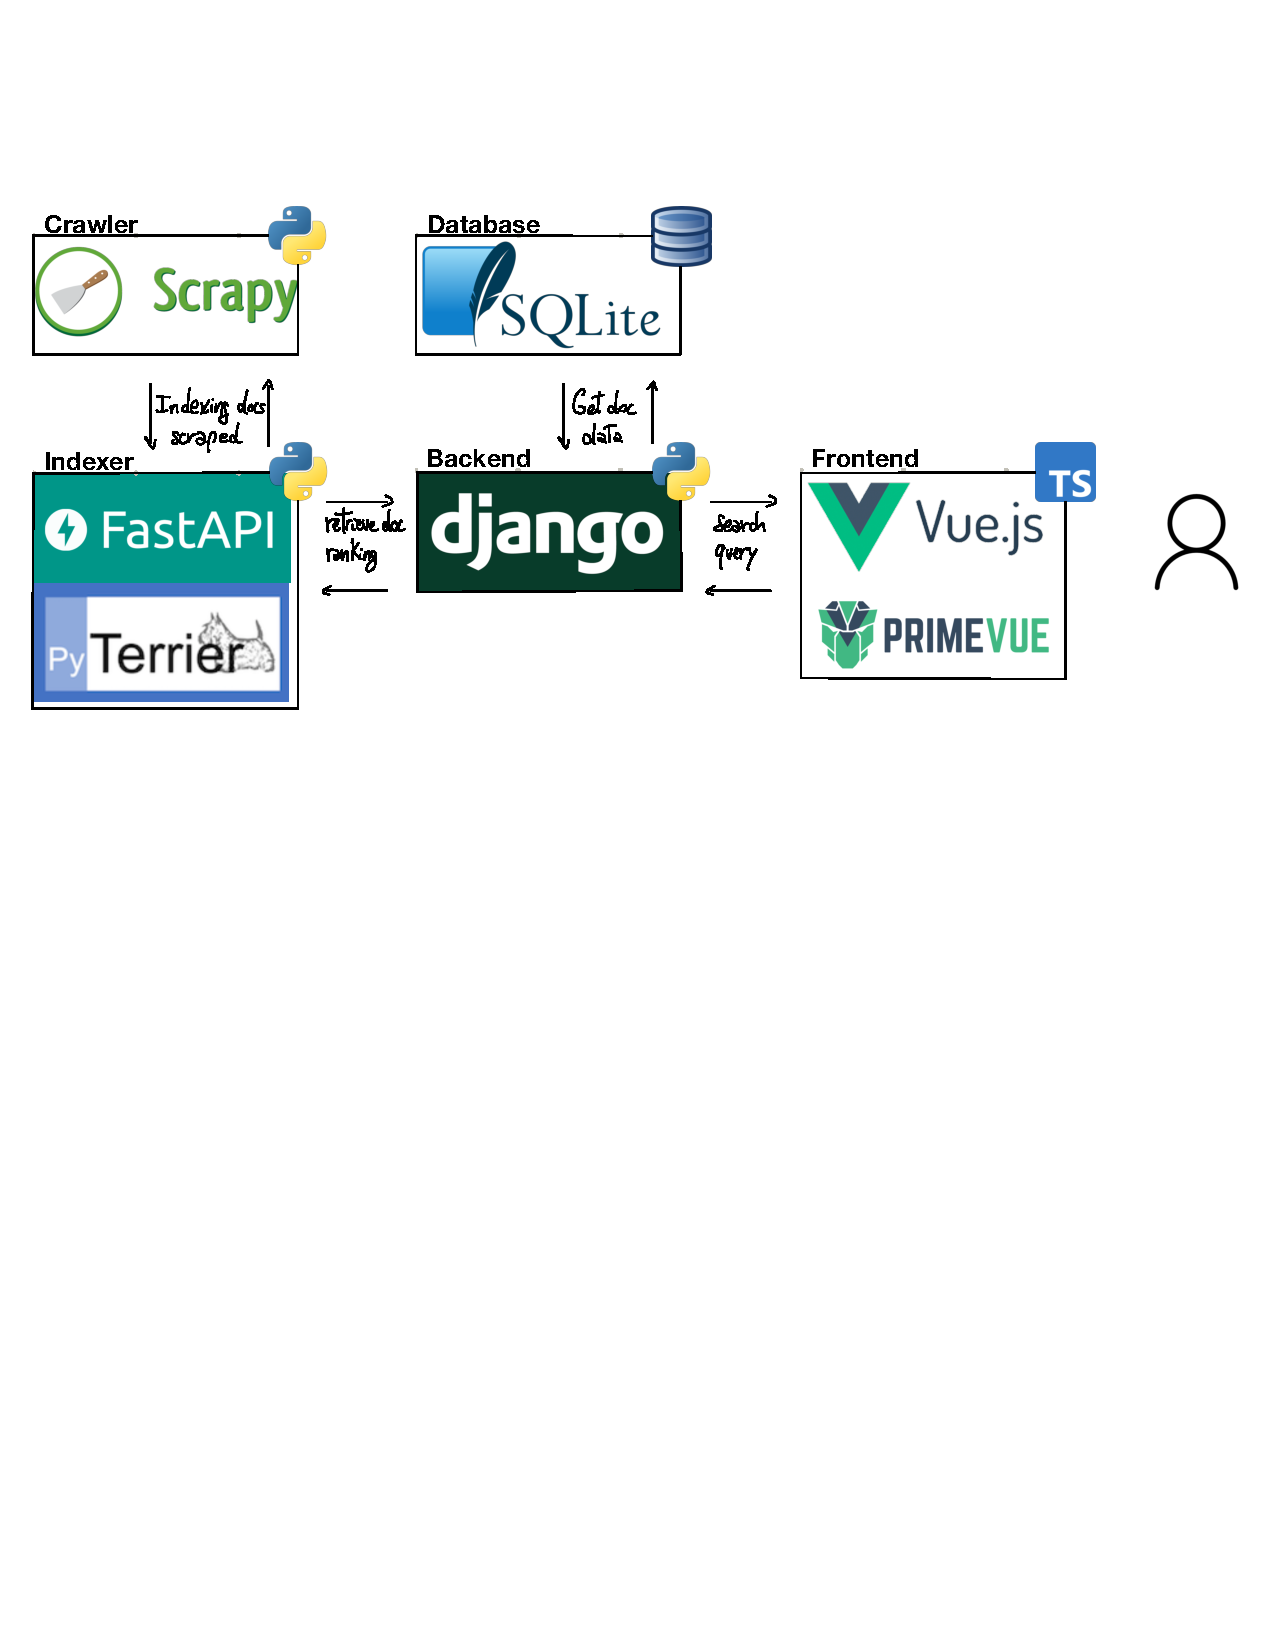
\includegraphics[width=\textwidth, trim={0cm 16cm 0cm 3cm}]{figures/architecture.pdf}
    \end{figure}

    The software components are: crawler, indexer, database, backend, frontend.\\
    RESTful APIs are used as interface for commucation between indexer-backend and backend-frontend.
    Communication between database-backend is encapsulated by Django,
    while crawler-indexer needs to be run manually through CLI prompt and file writing.

    \subsection{Technology Stack}
    Mandatory technologies to use for the project implementation: scrapy, pyterrier.
    Here below is listed the tech stack used with a short description and motivation of choice.

    \subsubsection{Scrapy}
    Scrapy is a Python application framework for crawling web sites and extracting structured data.
    It is used to initialize the crawling \& scraping process for a specified set of artworks.
    Crawling process is further discussed in section \ref{sec:crawling}.

    \subsubsection{PyTerrier}
    PyTerrier is a Python declarative platform for information retrieval experiments.
    It uses the Java-based Terrier information retrieval platform internally to support indexing and
    retrieval operations.
    Indexer process is further discussed in section \ref{sec:indexing}.

    \subsubsection{Django \& SQLite}
    Django is a
    FOSS\footnote{Free and Open Source}
    high-level Python web framework for rapid development and clean, pragmatic design.
    It takes care of much of the hassle of web development.\\
    By default, the Django configuration uses SQLite as database,
    which is the easiest choice of implementation already is included in Python.
    Backend functionality and interaction with database is detailed in Sections
    \ref{sec:backend}.

    \subsubsection{Vue.js 3 \& PrimeVue}
    The progressive javascript framework described as approachable, performant and versatile
    for building web user interfaces.
    It is an industry standard among the js component-based frameworks and it is used in courses
    since the 2\textsuperscript{nd} year of the bachelor.\\
    Together with PrimeVue, a complete UI suite for Vue.js, it elevates the web application with
    customizable, feature-rich UI components.
    %check responsivess
    Frontend design specifics are in Sections \ref{sec:frontend}, \ref{sec:ui}, \ref{sec:ux}.\\

    The search engine requirements are futher described, measured and discussed
    in the Evaluation Section \ref{sec:evaluation}.

    %%%%%%%%%%%%%%%%%%%%%%%%%%%%%%%%%%%%%%%%%%%%%%%%%%%%%%%%%%%%%%%%%
    \section{Crawling}\label{sec:crawling}
    It is part of \textbf{Indexing Process}, regarding \textbf{Text Acquisition}, in which the system
    identifies and stores documents for indexing.\\
    The purporse is to harness (relatively) bit text data characterized with the 5
    Vs\footnote{Volume, Variety, Velocity, Value, Veracity}
    located in previous mentioned web sites regarding for sale art.
    Among the 5 Vs, automating the Velocity attribute to keep track of the dynamic real-time data characterizing
    the art selling market was not possible:
    manual re-crawling of the spiders and inverted index re-creation is needed.
    Crawling through Scrapy parses text that is unstructed to group it in well-structured documents,
    allowing them to be easily indexed.
    The structure of each documents is:
    \vspace{-0.1cm}
    \begin{itemize}
        \setlength\itemsep{0.1em}
        \item author
        \item title
        \item price
        \item description
        \item categories
        \item image url reference
        \item post url reference
    \end{itemize}

    The extracted data is subsequently channeled into a \textit{.json} file specified at start.
    After all spiders have been run, every result is manually merged into the \textit{results.json} file.\\
    Our sample volume is around $\approx 8,500$ entries.
    To run crawling refer to project's \textit{README.md}.

    \section{Indexing}\label{sec:indexing}
    It is part of \textbf{Indexing Process},
    regarding \textbf{Text Transformation}, in which the system transforms documents into index terms,
    \textbf{Index Creation}, where index terms are employed to create data structures to support fast searching,
    and \textbf{Ranking and Retrieval}, which uses query and index to generate a ranked list of docs.\\
    The Pyterrier platform supports indexing and retrieval operations by employing shallow
    NLP\footnote{Natural Language Processing}
    techniques.\\
    The indexer served through a FastAPI server in \textit{crawler/index.py} file,
    returns a ranked list of documents in descending order of relevance probability $p \in [0,1]$,
    which is the optimal standard strategy justified by the
    \textbf{Probability Ranking Principle} [Robertson 77].
    The indexer creates the inverted index from the \textit{results.json} file containing the scraped documents.
    Characteristics of index:
    \vspace{-0.1cm}
    \begin{itemize}
        \setlength\itemsep{0.1em}
        \item Stemmer: Porter, algorithmic-basedd, Pyterrier's default
        \item Stopword: Pyterrier's default
        \item Tokenisation: English words, Pyterrier's default
    \end{itemize}

    The retrieval model is BM25: similarity-based model with ranked retrieval including
    TF\footnote{Term Frequency},
    IDF\footnote{Inverse Document Frequency}
    and sublinear TF transformation to avoid single term dominance.
    %Around x terms in the \textbf{lexicon}
    To run the indexer refer to project's \textit{README.md}.

    %%%%%%%%%%%%%%%%%%%%%%%%%%%%%%%%%%%%%%%%%%%%%%%%%%%%%%%%%%%%%%%%%
    \section{Retrieval}

    \subsection{Backend}\label{sec:backend}
    The backend relies on a SQLite database to store the main information about the documents,
    making it possible to retrieve the relevant ones following a call to the index.\newline
    The backend handles the two main fetches of the application:

    \begin{itemize}
        \item \textit{GET /api/documents/get-documents/\underline{query}/}:
              Endpoint facilitating the retrieval of relevant documents based on a provided \underline{query} string.
        \item \textit{GET /api/recommendation/get-recommended/}:
              Endpoint tasked with retrieving recommended artworks.
              By inputting a set of tags, it conducts a search within the index,
              returning all pertinent documents associated with the specified category tags.
    \end{itemize}

    The backend is the joint between the frontend and the indexer.
    It routes fetch request and, given a query, it returns the list of relevant documents with its main information
    by iterating through the database containing it for each artwork.

    \subsubsection{Automatic recommendation}\label{sec:recommender}
    The 2\textsuperscript{nd} API call is used to implement the \textit{recommender system}:
    the frontend keeps track of the categories as \textbf{browser traces} from the results given by user's queries.
    Then, the indexer receives such categories as query and give back a set of documents to the backend.
    This set is populated with its information stored in the database and it is finally given back to the frontend in
    the suggestions carousels.
    Essentially, once all the artworks related to the query have been retrieved,
    the frontend extracts from all these artworks the related tags,
    it chooses the ones with the higher frequency, fetches result using the API call and
    shows a maximum of 5 results related to each tag in a moving carousel
    It is a \textbf{Content-Based Information Filtering}:
    recommendation in such dynamic collection is individual to users based on interest and preferences inferred from
    previous user pseudo feedback, hence assuming top retrieved documents are relevant.
    At the end of each section the recommendations tags are cleaned i.e. page reload.

    % photo of carousel
    \begin{figure}[H]
        \centering
        \caption{Automatic Recommendation - Carousel}
        \label{fig:carousel}
        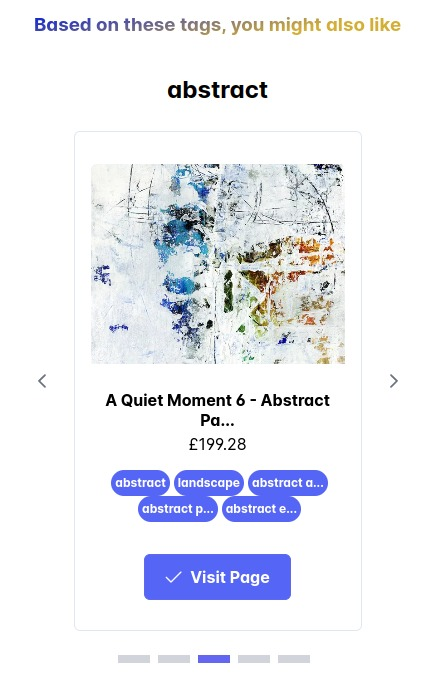
\includegraphics[width=0.3\textwidth, trim={0cm 0cm 0cm 0cm}]{figures/recommendation-carousel.jpeg}
    \end{figure}

    \subsection{Frontend}\label{sec:frontend}
    Part of \textbf{Query and Retrieval Process},
    regarding \textbf{User Interaction}, in which the system supports the creation of a query and display results.\\
    The frontend is the main part of the application, where all the features are implemented.
    For the interface, it has been chosen a simple layout shown in Figure \ref{fig:ui},
    consisting of only a search bar and a search button.
    Once the user performs the search, the aspect of the page changes, adding new components:

    \begin{figure}[H]
        \centering
        \caption{UI of the \textit{Art For Sale} project}
        \label{fig:ui}
        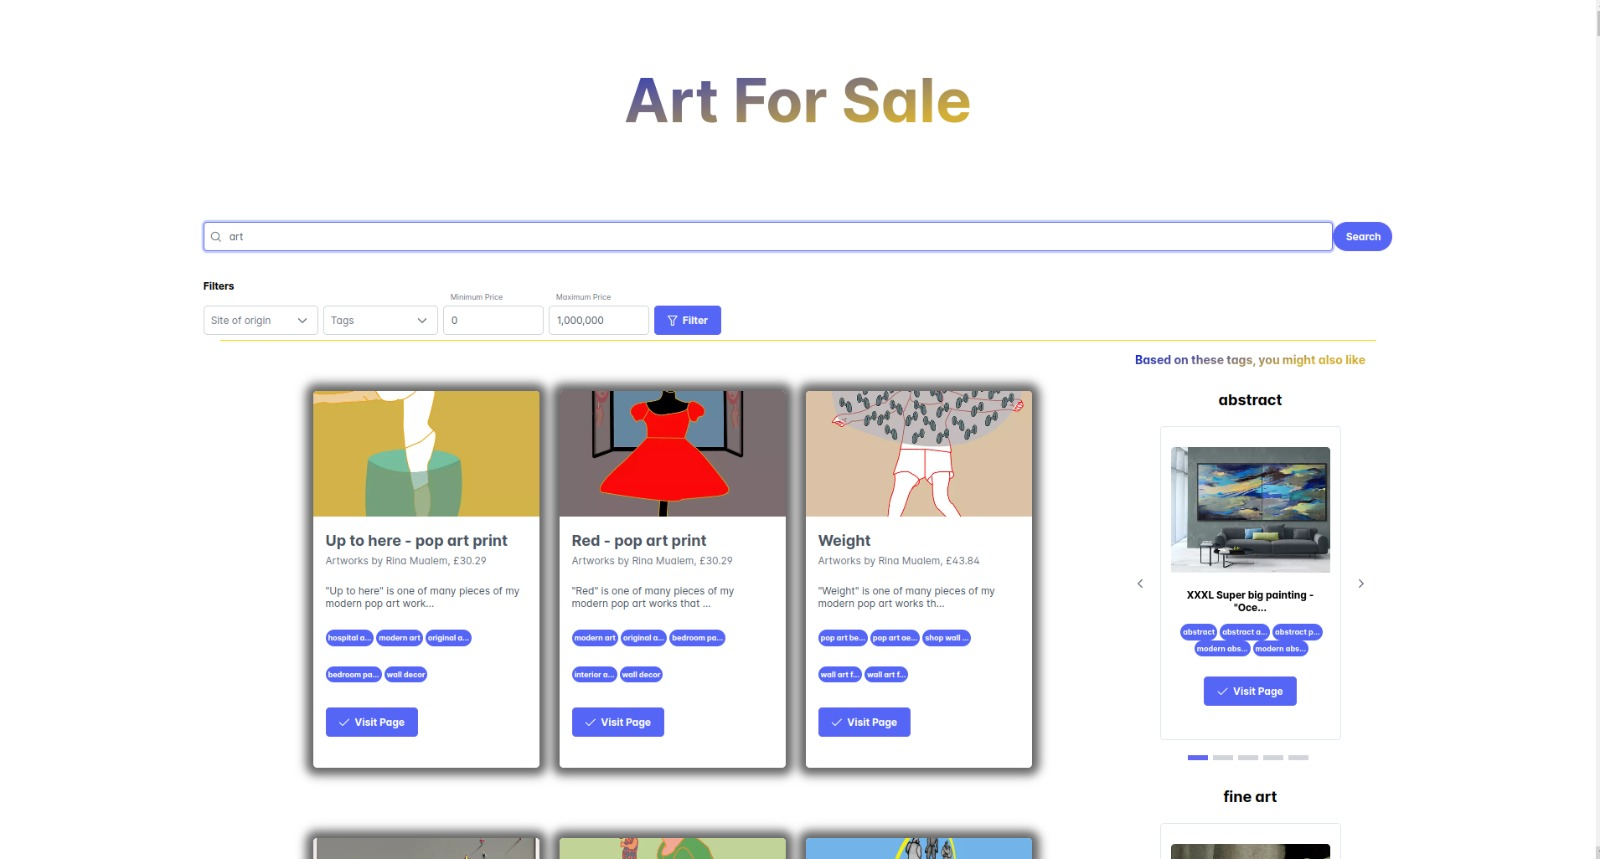
\includegraphics[width=\textwidth, trim={7cm 0cm 7cm 2cm}, clip]{figures/ui.jpeg}
    \end{figure}

    \begin{itemize}
        \item \underline{Filter selectors}: under the search bar there are filter selectors to control the obtained results
              according to 4 main characteristics:
              site of origin, minimum price, maximum price and category tag.
        \item \underline{Recommended Carousel}:
              At the right side of the page, the recommended carousel suggests results based on the most frequent tags
              of the resulted artworks.
              It shows a maximum of 5 results related to each tag in a moving carousel.
        \item \underline{Document tabular view}: retrieved artworks from the query are displayed in card components,
              following a tabular view as requested by the simple feature implemented.
              The card shows an insight of artwork image, author, title, price, short description and main tags,
              with a \textit{"Visit"} button that will bring the user to the page of that artwork in the original website.
    \end{itemize}

    \subsubsection{User Interface}\label{sec:ui}
    UI has been layed out following Jakob's 10 usability heuristics as much as possible, particularly:
    aesthetic and minimalist design, visibility of system status and consistency and standards.\\
    Norman's Emotional Design guidelines have been followed to obtain a UI gradient effect and minimalism similar
    to what is the user experience in Apple products, so users will feel confortable using it.

    \subsubsection{Filtering}\label{sec:filtering}
    The filtering features is implemented frontend side.
    If no filter is selected, then it simply shows all the results from the query.
    Otherwise, it checks:
    \begin{itemize}
        \setlength\itemsep{0.1em}
        \item price value range: check if the document value is between the min and max inserted
        \item web sites: check if the document origin url contains the selected website(s)
        \item category: the UI allows only to select a category from the ones already present in the result of your query
    \end{itemize}


    %%%%%%%%%%%%%%%%%%%%%%%%%%%%%%%%%%%%%%%%%%%%%%%%%%%%%%%%%%%%%%%%%
    \section{Evaluation}\label{sec:evaluation}
    Part of the \textbf{Query and Retrieval Process}, regarding \textbf{Evaluation}.\\
    \textbf{Effectiveness}: quality of results.
    Employing of \textbf{query expansion} was tested by always adding the \textit{art} keywork
    at the end of each search to get more results.
    This led to under-constrained query giving back not relevant results.
    The reason was due to the fact that for our specific set of concerns, hence documents, the word
    \textit{"art"} is an high frequency word, thus useless to achieve pertinency as explained by
    \textbf{Zipf's Law}.

    At start, every field was in a \textit{pandas.Series} and then given to the indexer but this lead to
    unsatisfying results: it seemed like only the first field (title) got indexed,
    giving an \textbf{over-constrained query} feeling where either no documents or no relevant ones were returned,
    Hence we decided to put every field into one big "blob" of text and then indexed that.\\
    \textbf{Efficiency}: response time and throughput.
    Since there is no pagination of results, all the list of relevant documents is sent and shown at once
    in the single page.
    This can lead to queries that give back hundred of documents and the response time to render them is high
    and has been partially leverage in the UX by adding a loader animation for retrieval,
    shown in Figure \ref{fig:loader}.

    \subsection{User Evaluation}
    Part of the \textbf{Relevance Feedback Process}, regarding \textbf{User Evaluation}.\\
    The conducted SUS modules are in \textit{docs/user-evaluation.pdf}.
    After the development, we have conduct an user evaluation on 5 different users using the SUS questionnaire.
    The SUS questionnaire is a 10-item questionnaire that measures the usability of a system.
    Each question is rated on a 5-point Likert scale, from strongly disagree to strongly agree.
    At the end of the questionnaire, we can compute the SUS score, which is a number between 0 and 100
    that indicates how usable the system is.
    We asked 5 users to use the system and fill the SUS questionnaire.
    While using the system we asked them to perform some tasks, such as searching for artworks,
    check the recommendations and use the filters.
    Sentiment analysis: all the users found the system intuitive and well-structured,
    without needing particular help to perform the various tasks.
    Once computed, we have obtained a 91.5\% SUS score.
    Given the results of the SUS questionnaire, we can say that the system is definitely usable
    and that the users are satisfied with it.

    \begin{figure}[H]
        \centering
        \caption{Loading animation while retrieving documents}
        \label{fig:loader}
        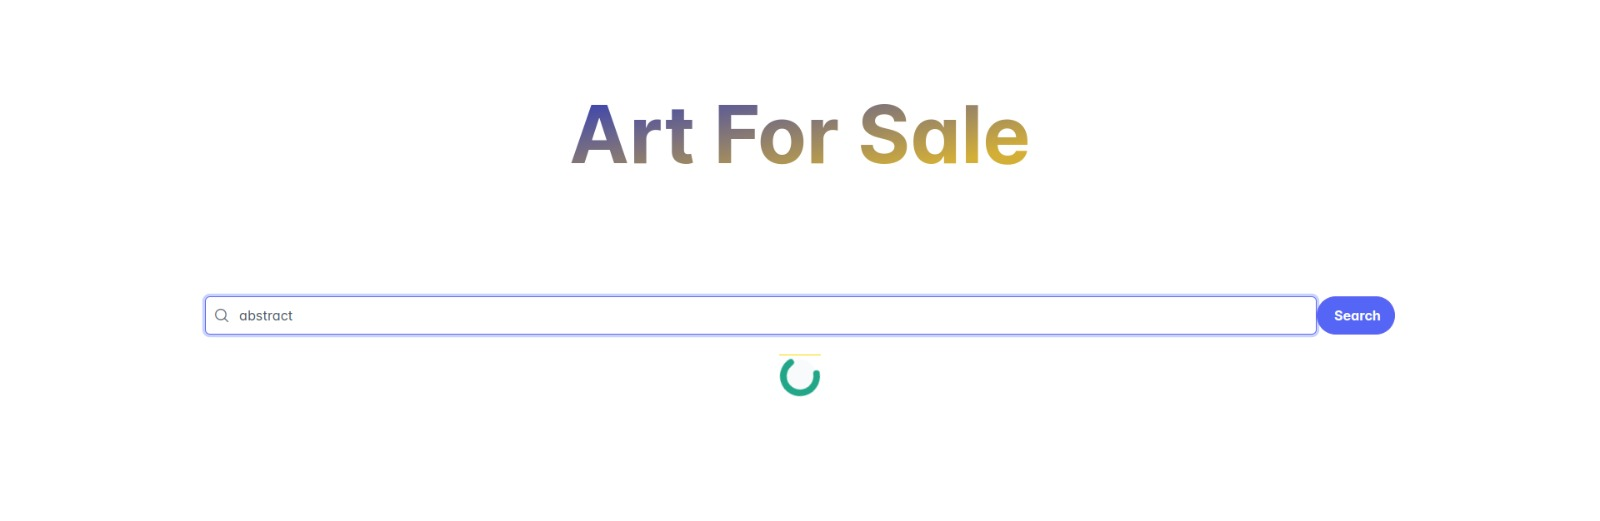
\includegraphics[width=\textwidth, trim={7cm 0cm 7cm 0cm}, clip]{figures/loading.jpeg}
    \end{figure}

    %%%%%%%%%%%%%%%%%%%%%%%%%%%%%%%%%%%%%%%%%%%%%%%%%%%%%%%%%%%%%%%%%
    \section{Limitations and Future Improvements}

    The project is a \textit{Text Retrieval} system at its current state.
    Since the type of data provided by artworks is not descriptive nor verbose,
    implementing \textit{Text Analysis} features becomes troublesome because lacking the large amounts of
    text data in order to discover interesting patterns buried in text.
    Nevertheless, \textit{Text Organization} implementation feasibility is high due to
    short well-structured categorized-based descriptions usually artwork documents have,
    allowing to connect and navigate scattered information.

    %%%%%%%%%%%%%%%%%%%%%%%%%%%%%%%%%%%%%%%%%%%%%%%%%%%%%%%%%%%%%%%%%
    \section{Conclusions}
    The project results is overall satifactory.
    We went for a couple iterations cycles to develop the whole stack and choosing the right tools aka frameworks
    allowed us to focus on the final result rather than non relevant technicalities.
    We had fun with deciding the technology stack to use and the architecture structure.
    We enjoyed the project freedom that allowed us to put in practice all the metholodogies
    learnt from this course and all the others we had during the bachelor.

    \section{References}\label{sec:references}
    \begin{itemize}
        \item \textit{ArtForSale} GitHub public repository: \url{https://github.com/JekxDevil/IR-ArtForSale}
        \item Course slides on iCorsi: \url{https://www.icorsi.ch/course/view.php?id=16928}
        \item \textit{Scrapy}: \url{https://docs.scrapy.org}
        \item \textit{Pyterrier}: \url{https://pyterrier.readthedocs.io}
        \item \textit{FastAPI}: \url{https://fastapi.tiangolo.com/}
        \item \textit{Django}: \url{https://www.djangoproject.com/}
        \item \textit{Vue.js 3}: \url{https://vuejs.org/}
        \item \textit{PrimeVue}: \url{https://primevue.org/}
    \end{itemize}

\end{spacing}
\end{document}
